%%%%%%%%%%%%%%%%%%%%%%%%%%%%%%%%%%%%%%%%%%%%%%%%%%%%%%%%%%%%%%%%%%%%%%
% Lớp 10 | Hàm số bậc hai và đồ thị | Hàm số bậc hai
% Dạng 0D3?2-5: Hàm số chứa dấu giá trị tuyệt đối
% Số câu: 2  (sinh tự động bởi tach_cau.py; từ nay thầy sửa trực tiếp file này)
%%%%%%%%%%%%%%%%%%%%%%%%%%%%%%%%%%%%%%%%%%%%%%%%%%%%%%%%%%%%%%%%%%%%%%

%%%%%%%%%%%%%%%% TRẮC NGHIỆM 4 PHƯƠNG ÁN %%%%%%%%%%%%%%%%

% nguồn: MaHoaNH_TracNghiem_Lop10
\begin{ex}%[0D3G2-5]%[ma:5ab15333]
	\immini{ 
	Cổng Arch tại thành phố St.Louis của Mỹ có hình dạng là một parabol. Biết khoảng cách giữa hai chân cổng bằng $162 \mathrm{\,m}$. Trên thành cổng, tại vị trí có độ  cao $43 \mathrm{\,m}$ so với mặt đất, người ta thả một sợi dây chạm đất. Vị trí chạm đất của đầu sợi dây này cách chân cổng $A$ một đoạn $10 \mathrm{\,m}$. Giả sử các số liệu trên là chính xác. Hãy tính độ cao của cổng Arch (chính xác đến phần chục)?
	\choice 
		{$175{,}6  \mathrm{\,m}$}
		{$197{,}5 \mathrm{\,m}$} 
		 {$210 \mathrm{\,m}$}
		{\True  $185{,}6 \mathrm{\,m}$}}
		{\vspace{-0.5cm} 
		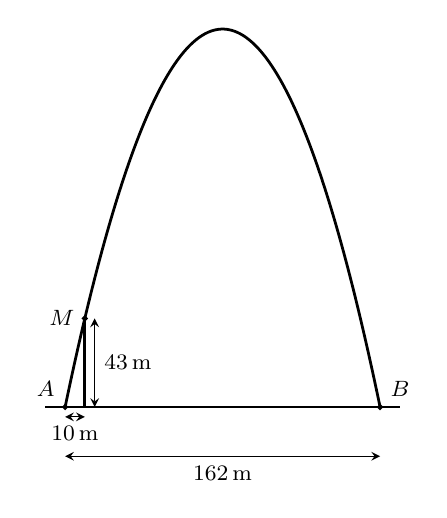
\begin{tikzpicture}[scale=0.25,line width=1pt,>=stealth,x=1mm,y=1mm]
				\draw (-10,0)--(0,0) node[above left] {\footnotesize $A$}  -- (160,0) node[above right]{\footnotesize $B$}--(170,0)
					 (10,45) node[left]{\footnotesize $M$};
				 \draw (10,0)--(10,45);
				 \draw[<->,thin](15,0)--(15,45) node[midway,right]{\footnotesize $43 \mathrm{\,m}$};
				\draw[<->,thin] (0,-5)--(10,-5) node[midway,below]{\footnotesize $10  \mathrm{\,m}$};
				 \draw[<->,thin] (0,-25)--(160,-25) node[midway,below]{\footnotesize $162 \mathrm{\,m}$};
				\draw[fill=black](0,0)  circle (2pt)
					 (10,45) circle (2pt)
					 (160,0) circle (2pt);
				\usepgflibrary{fpu} 
				\draw[smooth,samples=100,domain=0:160,/pgf/fpu,/pgf/fpu/output format=fixed] plot  (\x,{-0.03*(\x)^2+4.8*(\x)});
			\end{tikzpicture}
		 }
	\loigiai{ 
	 \immini{
		Đặt hệ trục toạ độ với $Axy$ như  hình vẽ.\\
		Xét  parabol $(P)\colon\,y=ax^2+bx+c$.\\
		Vì $M(10;43) \in (P)$ nên $100a+10b+c=43$.\hfill($ 1  $)\\
		Vì $A(0;0) \in (P)$ nên  $c=0$.\hfill($ 2 $)\\
		Vì $B(162;0)  \in (P)$ nên $162^2a+162b+c=0$.\hfill($ 3 $)\\
		 Giải hệ ($ 1 $), ($ 2 $), ($ 3 $) ta được $(P)\colon y=-\dfrac{43}{1520}x^2+\dfrac{3483}{760}x$.\\
		$(P)$ có trục đối xứng là  $x=81$.\\
		Suy ra chiều cao của cổng là  $y(81) \approx 185{,}607 \mathrm{\,m}$.
		 }
		{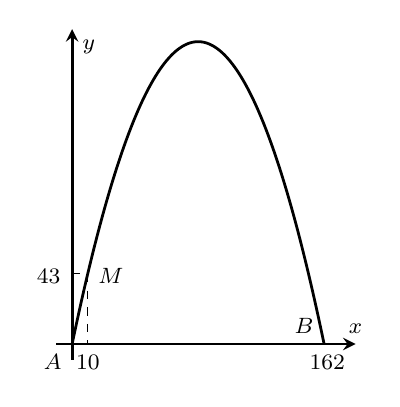
\begin{tikzpicture}[scale=0.2,line width=1pt,>=stealth,x=1mm,y=1mm]
		\draw (0,0) node[below left] {\footnotesize  $A$}
			(10,43) node[right]{\footnotesize  $M$}
			 (160,0) node[above left]{\footnotesize $B$};
		\draw[->] (-10,0)  -- (180,0) node [above] {\footnotesize$x$};
		\draw[->] (0,-10)  -- (0,200) node [below right] {\footnotesize$y$};
		\foreach \x/\xtext  in {10/10,162/162}
		\draw[shift={(\x,0)}]  (0pt,2pt)--(0pt,-2pt) node[below] {\footnotesize $\xtext$};
		 \foreach \y/\ytext in {43/43}
		 \draw[shift={(0,\y)}] (2pt,0pt)--(-2pt,0pt) node[left] {\footnotesize $\ytext$};
		\draw[dashed,thin]  (0,45)--(10,45)--(10,0);
		\usepgflibrary{fpu} 
		\draw[smooth,samples=100,domain=0:160,/pgf/fpu,/pgf/fpu/output format=fixed] plot (\x,{-0.03*(\x)^2+4.8*(\x)}); 
	\end{tikzpicture}
		} 
	} 
\end{ex}


%%%%%%%%%%%%%%%% TỰ LUẬN %%%%%%%%%%%%%%%%

% nguồn: MaHoaNH_TuLuan_Lop10
\begin{bt}%[0D3K2-5]%[ma:fbc36a7b]
	\immini{Một quân vua được  đặt trên một ô giữa
	bàn cờ vua. Mỗi bước di chuyển, quân vua được  chuyển
	sang một ô khác chung cạnh  hoặc chung đỉnh với ô đang
	 đứng (xem hình minh họa). Bạn An di chuyển quân vua
	ngẫu nhiên $3$ bước.  Tính xác suất để sau $3$ bước đi quân
	vua  trở về ô xuất phát?
	 }{
	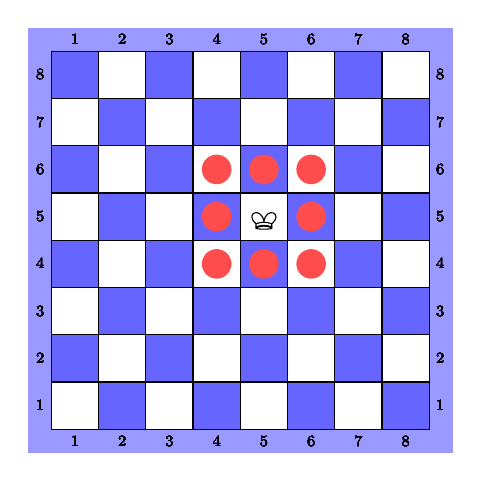
\begin{tikzpicture}[font=\footnotesize,line join=round,line cap=round,>=stealth]
			\begin{scope}[scale=.6]
				\tikzset{vua/.pic={ 
				 \def\a{1}
				\draw ([shift={(0,-\a/4)}]-\a/2,0)--(-\a/2,0)..controls ++ (140:1) and  ++(100:1)..(0,0.15)..controls ++(80:1) and ++(40:1)..(\a/2,0)--++(-90:\a/4)..controls++(-30:0.25) and++(-150:0.25)..(-\a/2,-\a/4);
				\foreach \d in  {0,\a/5,\a/4}{
					\draw[shift={(0,-\d)}](-\a/2,0)--(-\a/2,0)..controls++(20:0.15) and++(180:0.15)..(0,0.1)..controls++(0:0.15) and++(160:0.15)..(\a/2,0); 
					}}} 
					\tikzset{vitri/.pic={ 
				 \def\a{0.75}
				\draw[fill=red!70,draw=none,scale=.5](0,0)  circle (\a/2);
					}} 
				\fill[blue!40](-0.5,-0.5)  rectangle (8.5,8.5);
				\foreach  \i in{0,1,...,7}
				 \foreach \j in{0,1,...,7}
					{ 
				\pgfmathparse{mod (\i+\j,2)?  "blue!60": "white"}
				\fill[\pgfmathresult,draw=black](\i,\j) rectangle (\i+1,\j+1); 
				 \pgfmathsetmacro{\k}{int (\j+1)}
				\path (0,\j+0.5)  node[scale=.7,left]{\k}
					 (8,\j+0.5) node[scale=.7,right]{\k}
					(\j+0.5,0)  node[scale=.7,below]{\k}
					(\j+0.5,8) node[scale=.7,above]{\k}; 
				} 
				\path (4.5,4.35)  pic[scale=0.2]{vua};
				\foreach \x/\y in{5/5,4/5,3/5,3/4,3/3,4/3,5/3,5/4} 
				 \path[shift={(0.5,0.5)}](\x,\y) pic{vitri};
			\end{scope}
		\end{tikzpicture}
	} 
	 \loigiai{
		Gọi $\Omega$ là không gian mẫu. Từ vị trí của quân vua, cứ mỗi bước sẽ có $8$ vị trí mà quân vua có thể đi. Do đó $|\Omega|=8^3=512$.\\ 
		Gọi $A$ là biến cố: "sau $3$  bước quân vua về ô xuất phát".\\
		\begin{itemize}
			\item  TH1: đi theo hình tam giác vuông cân tại đỉnh vua ban đầu $4\cdot 2 = 8$ cách.
			\begin{center}
				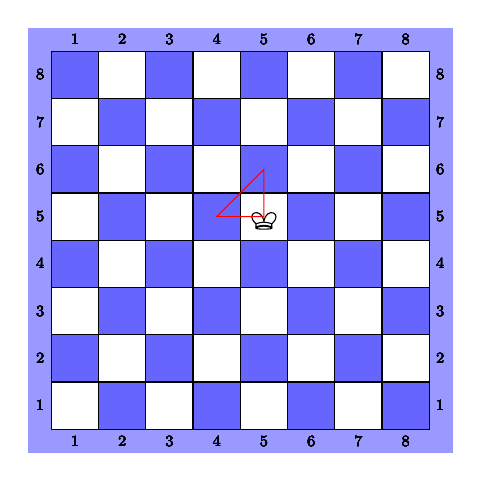
\begin{tikzpicture}[font=\footnotesize,line join=round,line cap=round,>=stealth]
						\begin{scope}[scale=.6]
						 \tikzset{vua/.pic={
						\def\a{1} 
						\draw ([shift={(0,-\a/4)}]-\a/2,0)--(-\a/2,0)..controls ++ (140:1) and ++(100:1)..(0,0.15)..controls ++(80:1) and ++(40:1)..(\a/2,0)--++(-90:\a/4)..controls++(-30:0.25) and++(-150:0.25)..(-\a/2,-\a/4); 
						 \foreach \d in {0,\a/5,\a/4}{
						 \draw[shift={(0,-\d)}](-\a/2,0)--(-\a/2,0)..controls++(20:0.15) and++(180:0.15)..(0,0.1)..controls++(0:0.15) and++(160:0.15)..(\a/2,0);
						 }}}
						\tikzset{vitri/.pic={ 
						\def\a{0.75} 
						 \draw[fill=red!70,draw=none,scale=.5](0,0) circle (\a/2);
						 }}
						\fill[blue!40](-0.5,-0.5) rectangle (8.5,8.5); 
						\foreach \i  in{0,1,...,7}
						\foreach \j  in{0,1,...,7}
						{ 
						\pgfmathparse{mod  (\i+\j,2)? "blue!60": "white"}
						\fill[\pgfmathresult,draw=black](\i,\j)  rectangle (\i+1,\j+1);
						\pgfmathsetmacro{\k}{int  (\j+1)}
						\path (0,\j+0.5) node[scale=.7,left]{\k} 
						(8,\j+0.5) node[scale=.7,right]{\k} 
						(\j+0.5,0)  node[scale=.7,below]{\k}
						(\j+0.5,8)  node[scale=.7,above]{\k};
						 }
						 \path (4.5,4.35) pic[scale=0.2]{vua};
						\draw[color=red]  (4.5,4.5)--(4.5,5.5)--(3.5,4.5)--(4.5,4.5);
						\end{scope}
					\end{tikzpicture}
			\end{center}
			\item TH2: đi theo hình tam giác vuông cân  tại đỉnh khác vua có $8\cdot 2= 16$ cách
			\begin{center}
				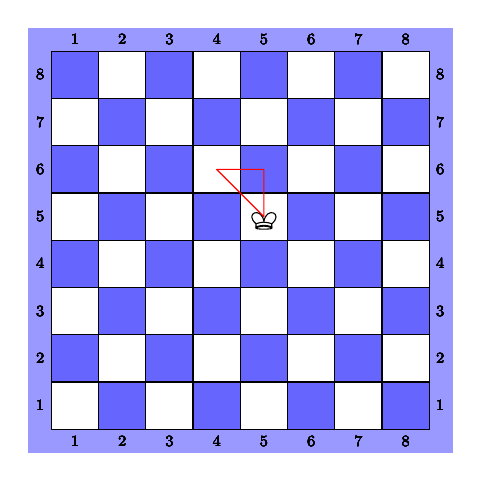
\begin{tikzpicture}[font=\footnotesize,line join=round,line cap=round,>=stealth]
						\begin{scope}[scale=.6]
						 \tikzset{vua/.pic={
						 \def\a{1}
						\draw  ([shift={(0,-\a/4)}]-\a/2,0)--(-\a/2,0)..controls ++ (140:1) and ++(100:1)..(0,0.15)..controls ++(80:1) and ++(40:1)..(\a/2,0)--++(-90:\a/4)..controls++(-30:0.25) and++(-150:0.25)..(-\a/2,-\a/4);
						\foreach  \d in {0,\a/5,\a/4}{
						\draw[shift={(0,-\d)}](-\a/2,0)--(-\a/2,0)..controls++(20:0.15) and++(180:0.15)..(0,0.1)..controls++(0:0.15)  and++(160:0.15)..(\a/2,0);
						 }}}
						 \tikzset{vitri/.pic={
						 \def\a{0.75}
						\draw[fill=red!70,draw=none,scale=.5](0,0) circle (\a/2); 
						 }}
						\fill[blue!40](-0.5,-0.5) rectangle  (8.5,8.5);
						\foreach  \i in{0,1,...,7}
						\foreach \j in{0,1,...,7} 
						{ 
						 \pgfmathparse{mod (\i+\j,2)? "blue!60": "white"}
						\fill[\pgfmathresult,draw=black](\i,\j) rectangle  (\i+1,\j+1);
						\pgfmathsetmacro{\k}{int  (\j+1)}
						\path  (0,\j+0.5) node[scale=.7,left]{\k}
						(8,\j+0.5) node[scale=.7,right]{\k} 
						(\j+0.5,0) node[scale=.7,below]{\k} 
						(\j+0.5,8)  node[scale=.7,above]{\k};
						 }
						\path  (4.5,4.35) pic[scale=0.2]{vua};
						 \draw[color=red] (4.5,4.5)--(4.5,5.5)--(3.5,5.5)--(4.5,4.5);
						\end{scope}
					\end{tikzpicture}
			\end{center}
		\end{itemize}
		Do  đó $|A|=8+16=24$ cách.\\
		Xác suất để sau $3$ bước đi quân vua về ô xuất  phát là $$P(A)=\dfrac{|A|}{|\Omega|}=\dfrac{24}{512}=\dfrac{3}{64}.$$
	} 
\end{bt}
